\chapter{Servidor de imágenes con tecnologías web }\label{cap.camserver}
En este capítulo se expone la creación de un nuevo driver para la plataforma JdeRobot. Este driver es un servidor de imágenes, al que se ha llamado CamServerWeb\footnote{\url{https://github.com/RoboticsURJC-students/2017-tfg-roberto-perez/tree/master/camserverWeb}}, obtenidas por una webcam (ya sea externa o interna del ordenador) de modo que cualquier aplicación externa pueda obtener las imágenes obtenidas.
\section{Diseño}
Este driver está diseñado con JavaScript y HTML como lenguajes de programación, WebRTC como biblioteca de captura de imágenes y ROS como middleware para la interconexión con los diferentes clientes. El driver puede ser ejecutado como una aplicación de escritorio usando el \textit{framework} Electron o como una página web usando un navegador. Gracias a esto se permite la ejecución multiplataforma sin necesidad de realizar modificaciones, lo que provee a este driver de una gran ventaja respecto a los tradicionales que se tenían, que están desarrollados para una única plataforma.  En la figura 6.1 se muestra el esquema de funcionamiento del driver.
\begin{figure}[H]
  \begin{center}
    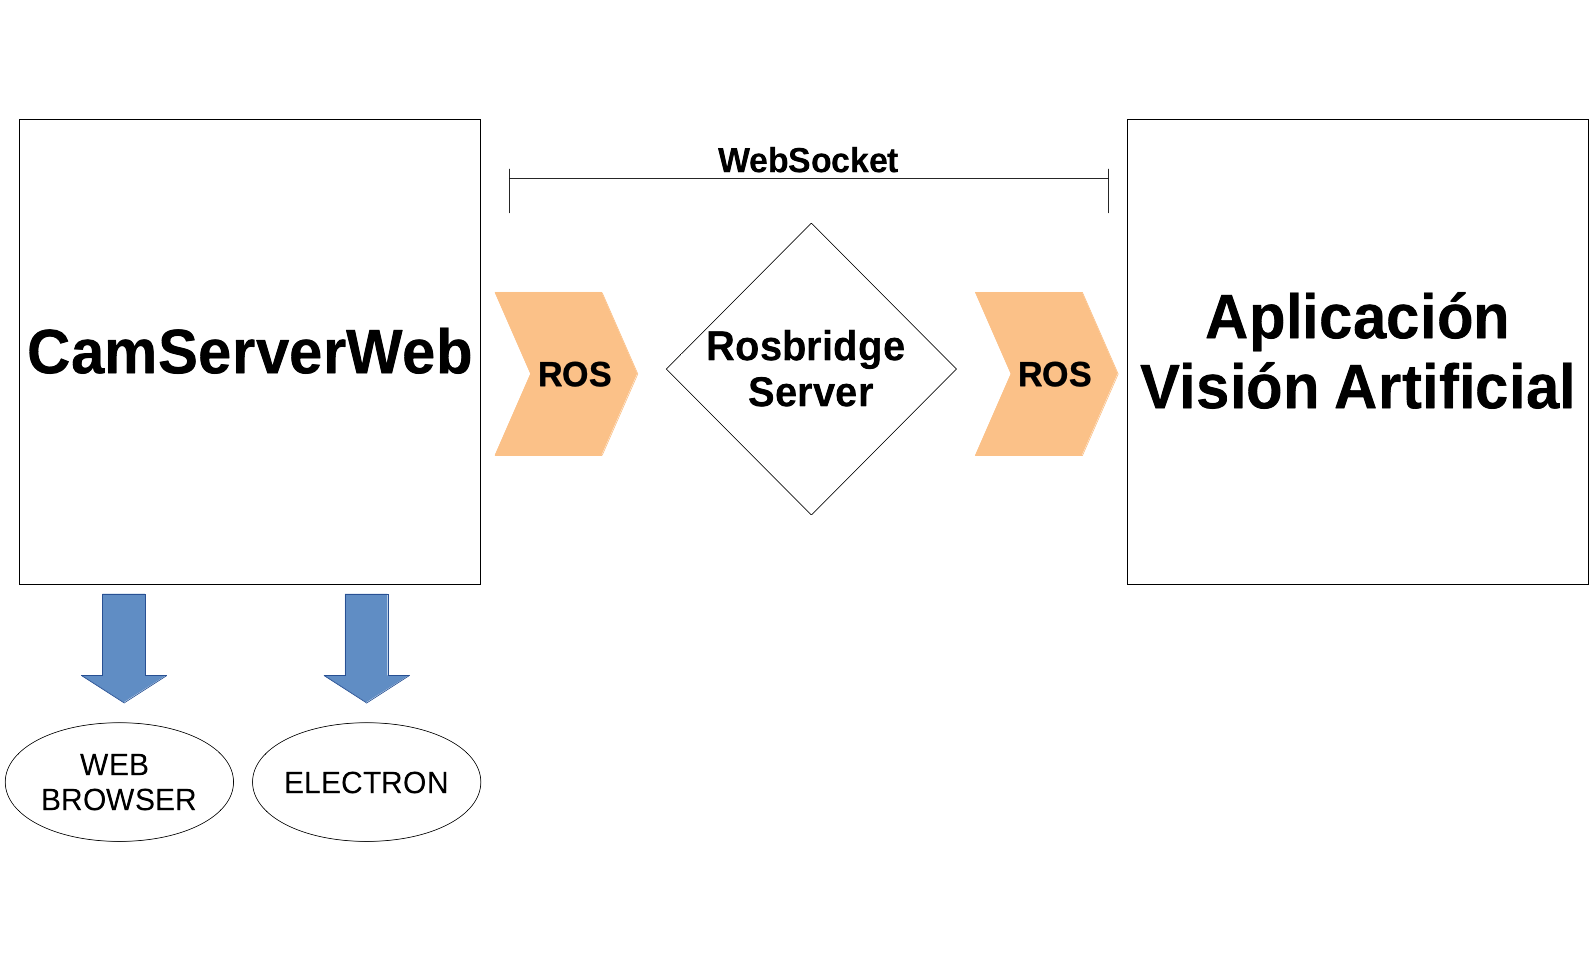
\includegraphics[width=0.8\textwidth]{figures/cajanegracamserver.png}
		\caption{Diseño del driver CamServerWeb}
		\label{fig.diseñocamserver}
		\end{center}
\end{figure}

Se puede apreciar en la figura 6.1 que entre el driver y la aplicación de visión artificial hay un servidor intermedio. Este servidor proporciona una capa de transporte WebSocket para realizar la conexión. En este caso permite la comunicación entre el servidor de imágenes y la aplicación de visión artificial que desea obtener las imágenes.

El driver cuenta con dos partes bien diferenciadas. La primera parte corresponde a la adquisición de las imágenes usando WebRTC para realizar la conexión con la fuente de video, y la segunda parte es la encargada de realizar la conexión mediante ROS y el posterior envío de los mensajes mediante los \textit{Publisher} de ROS para que sean recibidos por la aplicación de visión artificial. Gracias al uso de ROS se posibilita que la aplicación de visión artificial esté desarrollada en cualquier lenguaje de programación y ejecutada en cualquier dispositivo ubicado en cualquier lugar del mundo. Finalmente, el driver cuenta con una interfaz gráfica de apoyo para realizar la configuración en tiempo de ejecución. Esta estructura se puede observar en la figura 6.2.
\begin{figure}[H]
  \begin{center}
    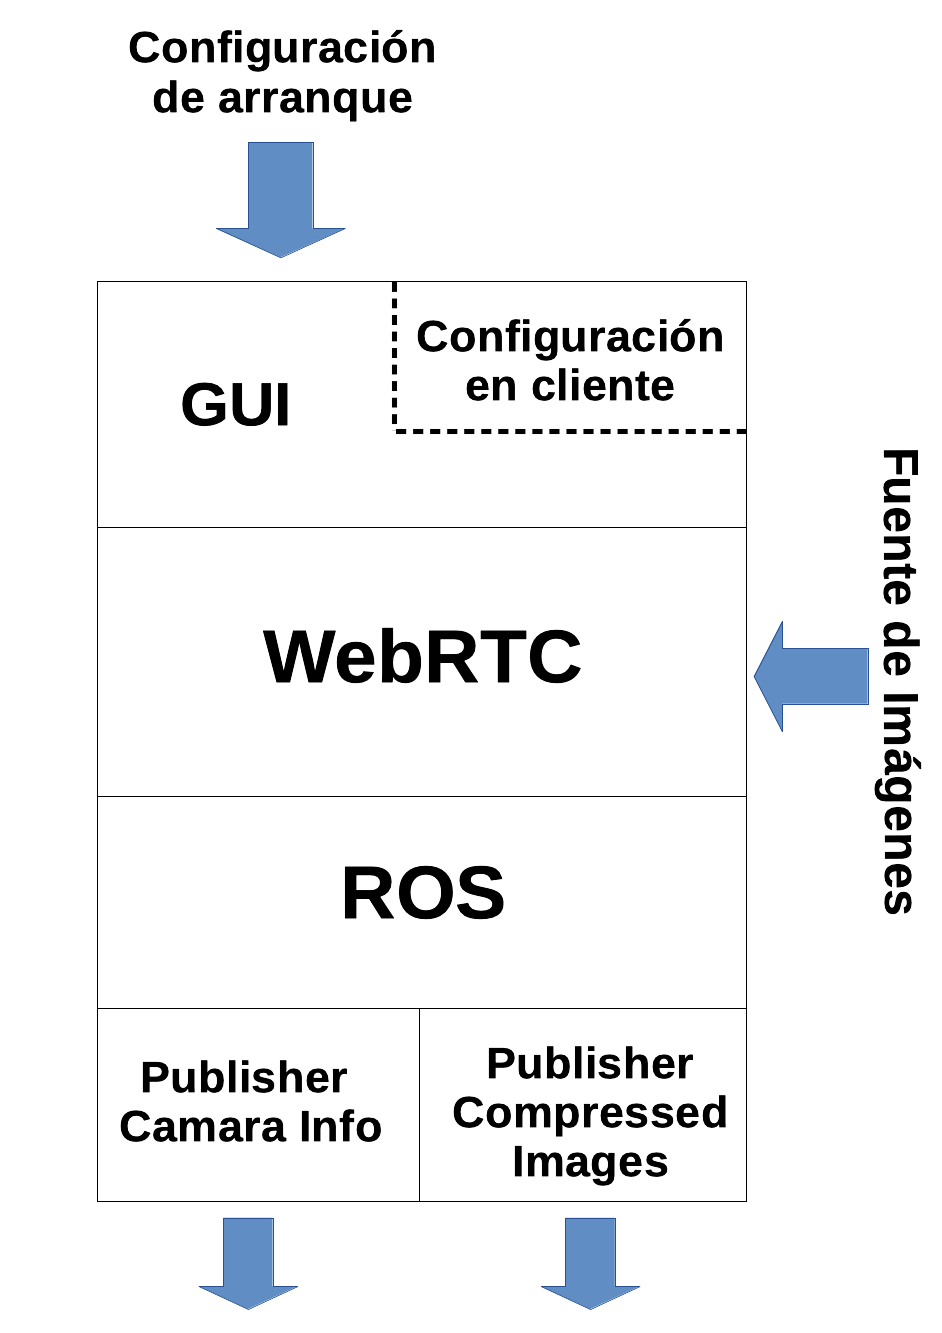
\includegraphics[width=0.8\textwidth]{figures/cajablancacamserver.png}
		\caption{Estructura interna de CamServerWeb}
		\label{fig.estructuracamserver}
		\end{center}
\end{figure}

\section{Adquisición y preparación de imágenes}
Para la obtención de las imágenes se hace uso del proyecto de código abierto WebRTC, que permite la captura y transmisión en tiempo real de audio, video y datos.
Mediante WebRTC se obtienen las imágenes de una cámara utilizando muy pocas líneas de código, lo que facilita enormemente el trabajo. El único problema que se ha tenido que solucionar, es el formato en el que se obtienen esas imágenes que es incompatible con ROS, por lo que se han tenido que llevar a cabo modificaciones en el formato de la imagen.

Lo primero que el driver debe realizar es recopilar todos los dispositivos conectados al ordenador y separar los dispositivos de video, que son los que realmente interesan. Para lograrlo, se utiliza el api \texttt{Navigator} de WebRTC, proporcionándo el objeto \texttt{navigator.mediaDevices}, al cual si le añadimos \texttt{.enumerateDevices().then(function (devices)\{\})}, obtenemos todos los dispositivos multimedia conectados al ordenador donde se está ejecutando. Una vez que se tienen todos los dispositivos, simplemente interesan capturadores de video, es decir, serán aquellos cuyo tipo es de entrada de video (en el código sería un condicional \texttt{if (devices.kind == "videoinput")\{\})}. La lista de dispositivos se muestra en el menú de configuración, mediante un campo desplegable, como se muestra en la figura 6.3.
 \begin{figure}[H]
  \begin{center}
    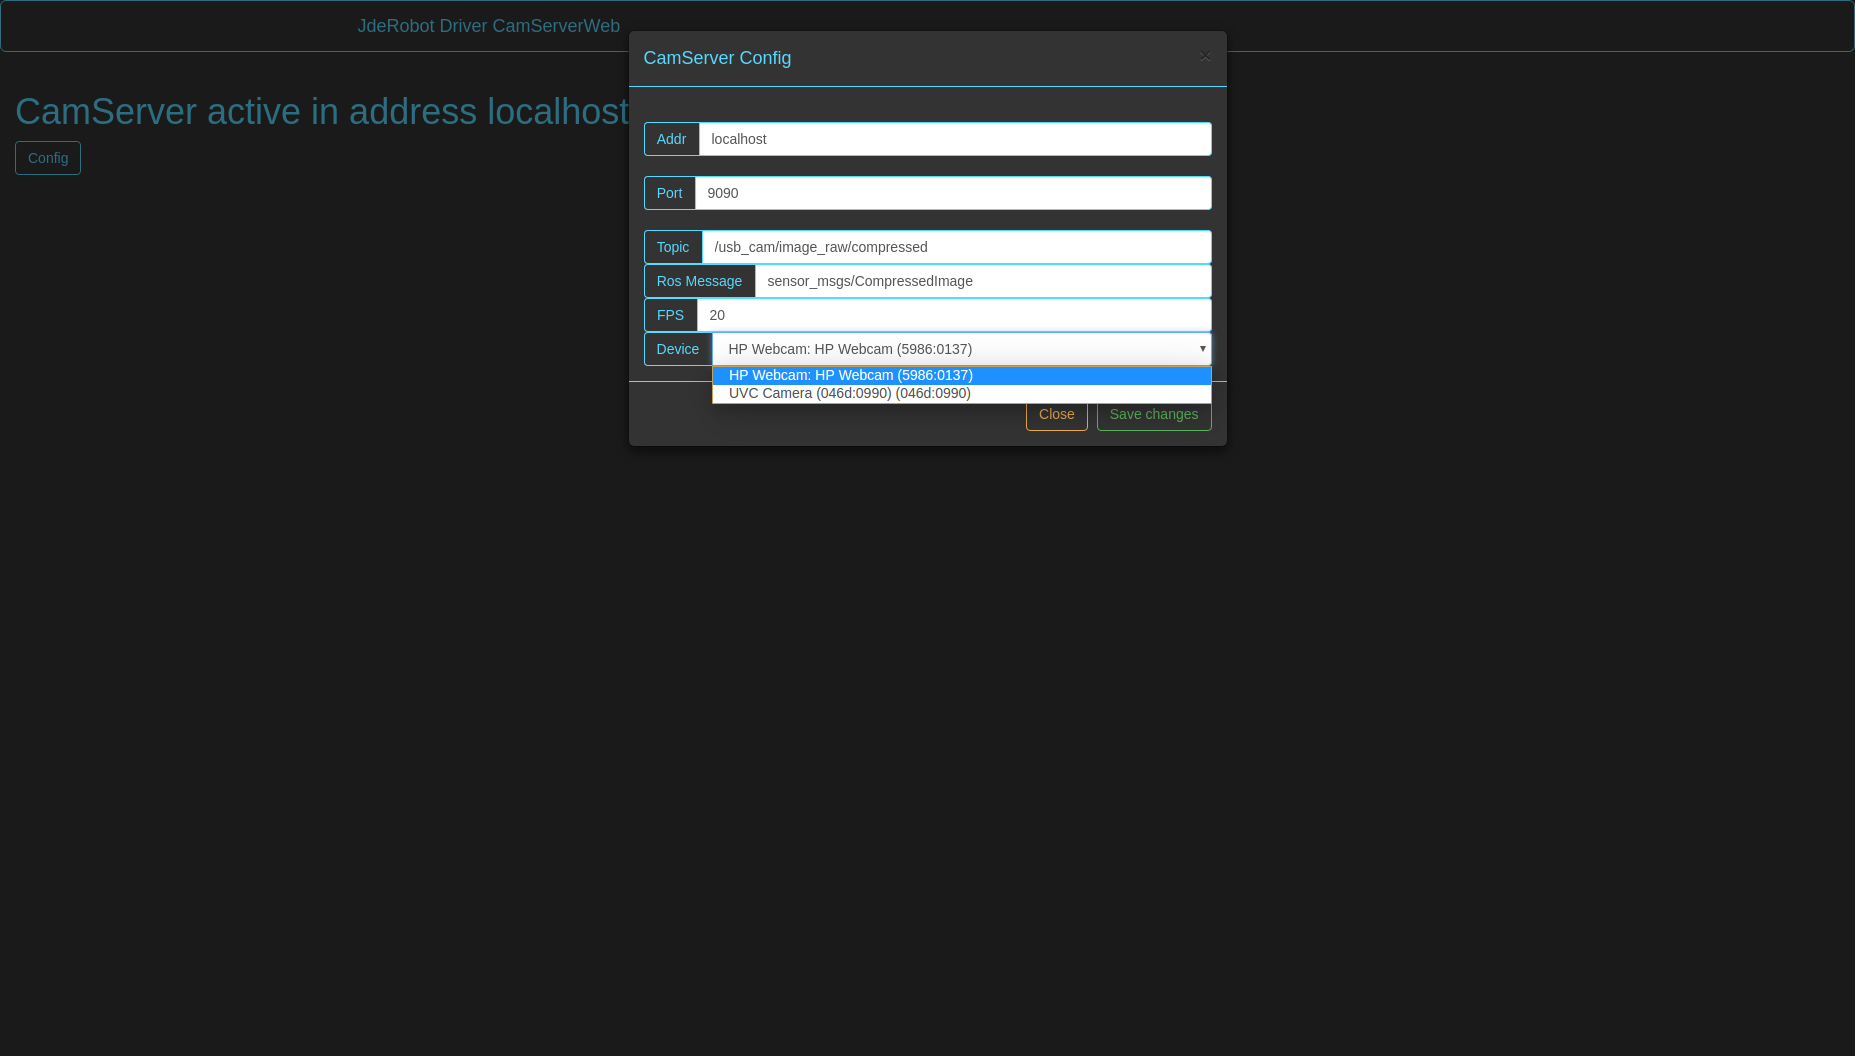
\includegraphics[width=0.8\textwidth]{figures/devicecamserver.png}
		\caption{Selector del dispositivo de entrada de video}
		\label{fig.devicecamserver}
		\end{center}
\end{figure}
Una vez que se selecciona el dispositivo que vamos a utilizar para adquirir las imágenes, hay que conectarse a él. Para esta conexión se vuelve a utilizar la API de WebRTC, \texttt{Navigator} y el objeto \texttt{Navigator.mediaDevices}, sin embargo en esta ocasión utilizamos el método \texttt{navigator.mediaDevices.getUserMedia(constraints).then(function(stream) \{\})}, donde \texttt{constraints} define los dispositivos multimedia (en este caso el dispositivo de entrada de video escogido) y \texttt{stream} es el flujo de datos obtenido de ellos.

Este flujo de datos está en el formato \texttt{MediaStream}, el cual no es apto para ser enviado o visualizado, por tanto es necesario realizar una conversión. Para realizar la conversión, se utiliza el elemento de HTML \texttt{Canvas} y el método JavaScript asociado a este elemento \texttt{toDataURL()}. Este método devuelve un \texttt{data URI} (URLs prefijados que permiten a los creadores de contenido incorporar pequeños archivos en línea en los documentos) que contiene una representación de la imagen en el formato especificado por el parámetro \texttt{type}, tomando en nuestro caso el valor \texttt{image/jpeg}, para obtener las imágenes en el formato comprimido jpeg. Todo está contenido en un canvas virtual, ya que no se mostrará en ningún lugar y únicamente se utiliza como pasarela entre el API de WebRTC y el envío de las imágenes.

\section{Conexiones}
En esta sección se explica cómo se realiza la conexión tipo ROS con la aplicación de visión artificial y el posterior envío de imágenes mediante un \textit{Publisher} de ROS. 

\subsection{Establecimiento de la conexión}
Para realizar la conexión es necesario el uso de la biblioteca \texttt{roslibjs} y que se ha explicado en capítulos anteriores. Esta biblioteca proporciona todo el código necesario para realizar la conexión, indicando si se ha realizado correctamente o a si ha ocurrido algún error. Para realizar la conexión, la biblioteca \texttt{roslibjs} proporciona el objeto \texttt{ROSLIB.Ros}, y el método proporcionado por este objeto, \texttt{ros.on}. El código para establecer la conexión se muestra en el cuadro 6.1.
\begin{lstlisting}[caption= Establecer conexión con ROS, label=cod.conexionRosCamserver]
ros = new ROSLIB.Ros();
ros = new ROSLIB.Ros({
            url : "ws://IP:Puerto"
 });
\end{lstlisting}
En este código se indica que la conexión se hace utilizando un canal de comunicación WebSocket, y la IP y puerto por la que se transmite. De esta forma ya se habrá establecido la conexión ROS, pero aún hay que definir el tipo de mensaje a enviar y a través de qué etiqueta de ROS (\textit{topic} de ROS) pueden conectarse las diferentes aplicaciones de visión artificial que deseen obtener las imágenes que se transmiten.

\subsection{Estructura de los mensajes}
El tipo de mensaje que vamos a utilizar para el envío es el tipo predefinido en el API de ROS, \texttt{sensor\_msgs/CompressedImage}. El motivo de esta elección es que las imágenes se obtienen en formato comprimido jpeg, tal y como se ha explicado en la sección anterior. Sin embargo, este tipo de mensaje no envía información acerca del tamaño de la imagen (altura y anchura), por lo que es necesario enviar otro mensaje adicional para completar esta información. Este mensaje de apoyo es de tipo \texttt{sensor\_msgs/CameraInfo} y transmitirá toda la información sobre la cámara (altura, anchura, etc). 

Para definir estos dos mensajes se utiliza el objeto proporcionado por la biblioteca \texttt{roslibjs}, \texttt{ROSLIB.Topic}. A este objeto se le deben introducir como parámetros el objetos \texttt{ROSLIB.Ros} generado para realizar la conexión, el nombre del \textit{topic} y el tipo de mensaje, por lo que se genera el \textit{Publisher} para servir las imágenes y la información de la cámara mediante el código del cuadro 6.2.
\begin{lstlisting}[caption= Estructura de los mensajes, label=cod.estrucuturamensajes]
var imagenTopic = new ROSLIB.Topic({
	ros:ros, 
	name: config.Topic, 
	messageType : "sensor_msgs/CompressedImage Message"})
	
var cameraInfo = new ROSLIB.Topic({
         ros: self.ros,
         name : "/usb_cam/camera_info",
         messageType: "sensor_msgs/CameraInfo"
       })

\end{lstlisting}

\subsection{Creación de los mensajes y publicación}
Definidos los tipos de mensajes y establecida la conexión, el siguiente paso es transmitir los mensajes. Para ello se deben crear los mensajes con la información que se desea transmitir con el \textit{Publisher}, utilizando de nuevo un objeto definido en la biblioteca \texttt{roslibjs}, \texttt{new ROSLIB.Message}. Para crear este objeto se debe pasar por parámetros el contenido que se quiere que tenga el mensaje, siempre cumpliendo las especificaciones definidas para cada tipo de mensaje que están definidas en la documentación de ROS\footnote{\url{http://wiki.ros.org/common_msgs}}. En este caso, para definir los dos mensajes que se transmiten se hara mediante el código del cuadro 6.3.
\begin{lstlisting}[caption= Definición del mensaje para las imágenes, label=cod.definicionmensajeimg]
 var videomensaje = new ROSLIB.Message({
 	format : "jpeg", 
	data : data.replace("data:image/jpeg;base64,", "")
	})

\end{lstlisting}
Del código del cuadro 6.3 cabe destacar que \texttt{data} corresponde a los datos obtenidos mediante el método \texttt{toDataURL} indicado en la sección 6.2, remplazando la cabecera donde se indica el formato, ya que se indica en el propio mensaje mediante \texttt{format}. 

Para el mensaje donde se transmite la información de la cámara se usa el código del cuadro 6.4.

\begin{lstlisting}[caption= Definición del mensaje para la información de la cámara, label=cod.definicionmensajeinfo]
var camarainfo = new ROSLIB.Message({
	height: imagen.height,
	width: imagen.width})

\end{lstlisting}
Una vez creados los mensajes, solo falta publicarlos, lo que se consigue de una manera sencilla mediante el código que se muestra en el cuadro 6.5.
\begin{lstlisting}[frame=single]
imageTopic.publish(imageMessage);
cameraInfo.publish(infoMessage);
\end{lstlisting}

Se puede apreciar fácilmente que lo que se está realizando es publicar los dos mensajes creados mediante la estructura definida anteriormente. 
Finalmente, es necesario enviar de una manera periódica estos mensajes, ya que con lo indicado anteriormente, únicamente se está enviando un mensaje de cada categoría. 
Para crear un envío periódico, se hace uso del método de JavaScript \texttt{SetInterval()}. Este método llama a una función o evalúa una expresión cuando pase un intervalo de tiempo (en milisegundos), que se indica en la llamada al método junto a la función que se quiere ejecutar cuando se cumpla el citado intervalo.

\section{Configuración}
Para configurar el driver se ofrecen dos posibilidades:
\begin{itemize}
\item Mediante el uso de un fichero con formato ``YAML'', al igual que en resto de herramientas de este trabajo. 
\item Mediante el menú de configuración incorporado en la interfaz gráfica.
\end{itemize}
El primer método realiza la configuración inicial del driver, ya que se configura al arrancar el driver. El segundo método permite realizar la configuración del driver durante la ejecución del mismo, ofreciendo la posibilidad de reconfigurar en tiempo de ejecución sin que sea necesario cerrar y volver a lanzar el driver.

Los parámetros configurables son los siguientes:
\begin{itemize}
\item Dirección IP. Por defecto es localhost.
\item Puerto. Por defecto será 9090.
\item \textit{Topic} al que se registran los clientes. Por defecto es \texttt{/usb\_cam/image\_raw/compressed}
\item Formato del mensaje. Por defecto es \texttt{sensor\_msgs/CompressedImage}
\item \textit{Framerate}. Por defecto son 20 fotogramas por segundo.
\item Fuente de video. Por defecto es la primera fuente detectada por WebRTC. Este parámetro únicamente puede ser configurado mediante la configuración en tiempo de ejecución.
\end{itemize}

\subsection{Interfaz gráfica}
La interfaz está realizada mediante HTML y Bootstrap, siguiendo el modelo del resto de aplicaciones web de la plataforma JdeRobot.
\begin{figure}[H]
  \begin{center}
    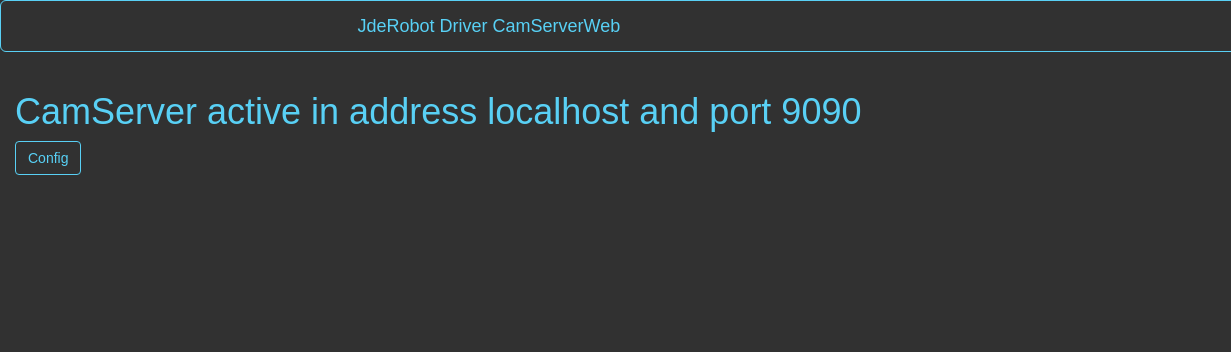
\includegraphics[width=0.8\textwidth]{figures/Interfazcamserver.png}
		\caption{Interfaz gráfica del driver}
		\label{fig.interfazcamserver}
		\end{center}
\end{figure}
La configuración se realiza gracias a un menú desplegable mediante la pulsación de un botón y una vez que se pulse el botón guardar, se almacena la nueva configuración para realizar las conexiones. Este menú se puede apreciar en la figura 6.5.
 \begin{figure}[H]
  \begin{center}
    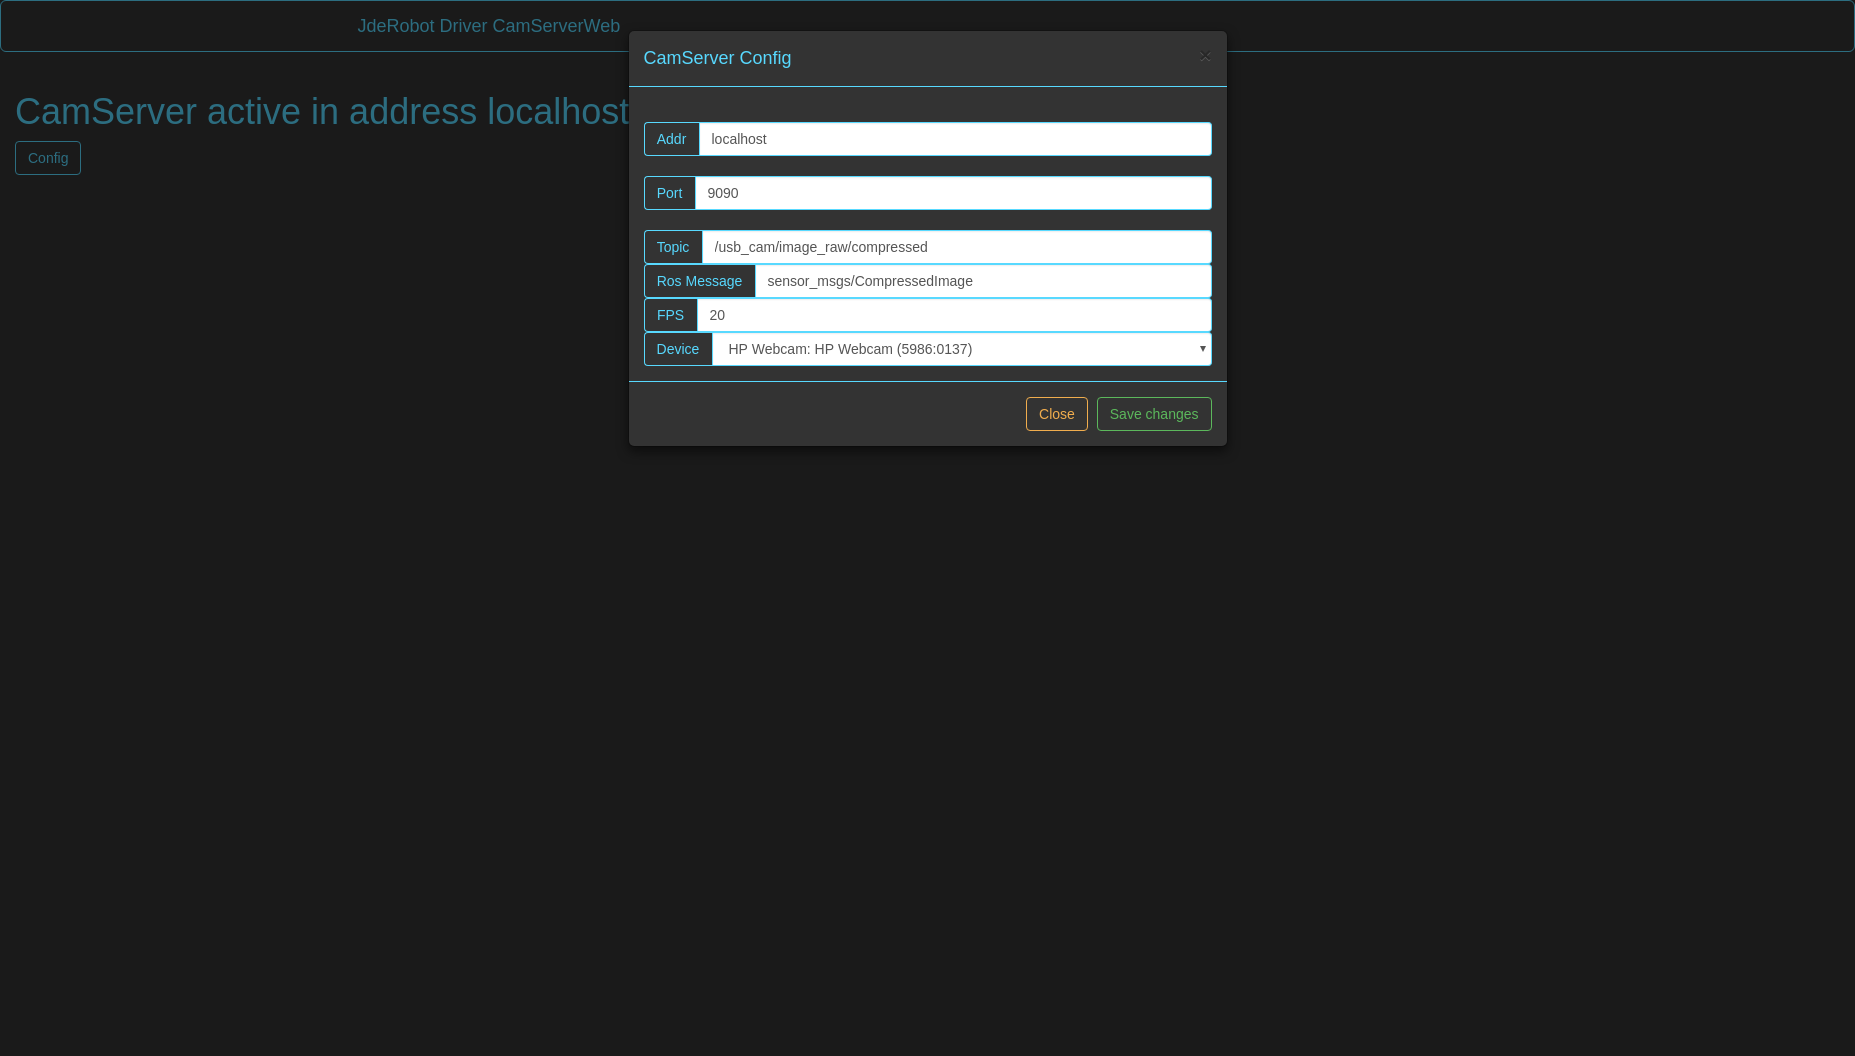
\includegraphics[width=0.8\textwidth]{figures/configcamserver.png}
		\caption{Menú de configuración del servidor de imágenes}
		\label{fig.configcamserver}
		\end{center}
\end{figure}

\section{Experimentos}
Como se ha visto anteriormente, el driver puede ejecutarse a través de dos vías: Electron y Node.js. La preparación para que funcione correctamente es la misma para ambas vías, siendo la única diferencia la forma de ejecutar el driver.

En un primer terminal o consola se debe ejecutar el servidor intermedio de ROS.

\begin{lstlisting}[caption= Ejecución del servidor intermedio, label=cod.servidorintermedio]
#>roslaunch rosbridge_server rosbridge_websocket.launch
\end{lstlisting}
En un segundo terminal se ejecutará el driver.
\begin{itemize}
\item 
Como aplicación web utilizando Node.js\footnote{\url{https://www.youtube.com/watch?v=taQzWUbYp-s}}
\end{itemize}
\begin{lstlisting}[caption= Ejecución con Node.js, label=cod.nodejs]
#>node run.js
Se arranca el navegador y se introduce la URL http://localhost:7777/
\end{lstlisting}
\begin{itemize}
\item 
Como aplicación de escritorio con Electron\footnote{\url{https://www.youtube.com/watch?v=3PTJyvtEaDE}}
\end{itemize}
\begin{lstlisting}[caption= Ejecución con Electron, label=cod.electron]
#>npm install
#>npm start
\end{lstlisting}
En ambos casos debemos configurar el driver para que se conecte con el servidor intermedio, en la imagen 4.5 muestra una posible configuración del driver.
\begin{figure}[H]
  \begin{center}
    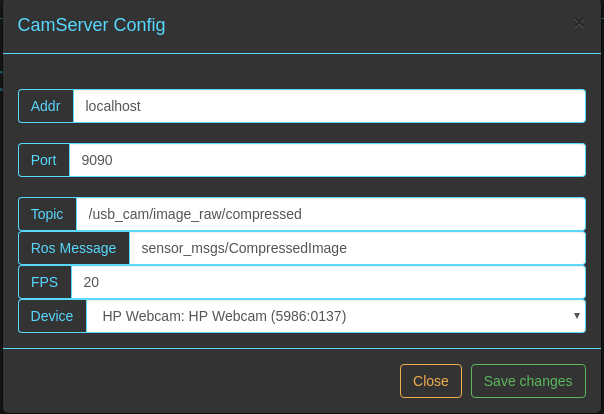
\includegraphics[width=0.8\textwidth]{figures/configcamservertest.png}
		\caption{Ejemplo de configuración del driver}
		\label{fig.esquemacamserver}
		\end{center}
\end{figure}
Finalmente, para verificar que está funcionando correctamente, en un tercer terminal lanzaremos la herramienta \texttt{rqt\_image\_view}, facilitada por ROS para visualizar imágenes enviadas a través de un mensaje de ROS, que hará la función de cliente.

\begin{figure}[H]
  \begin{center}
    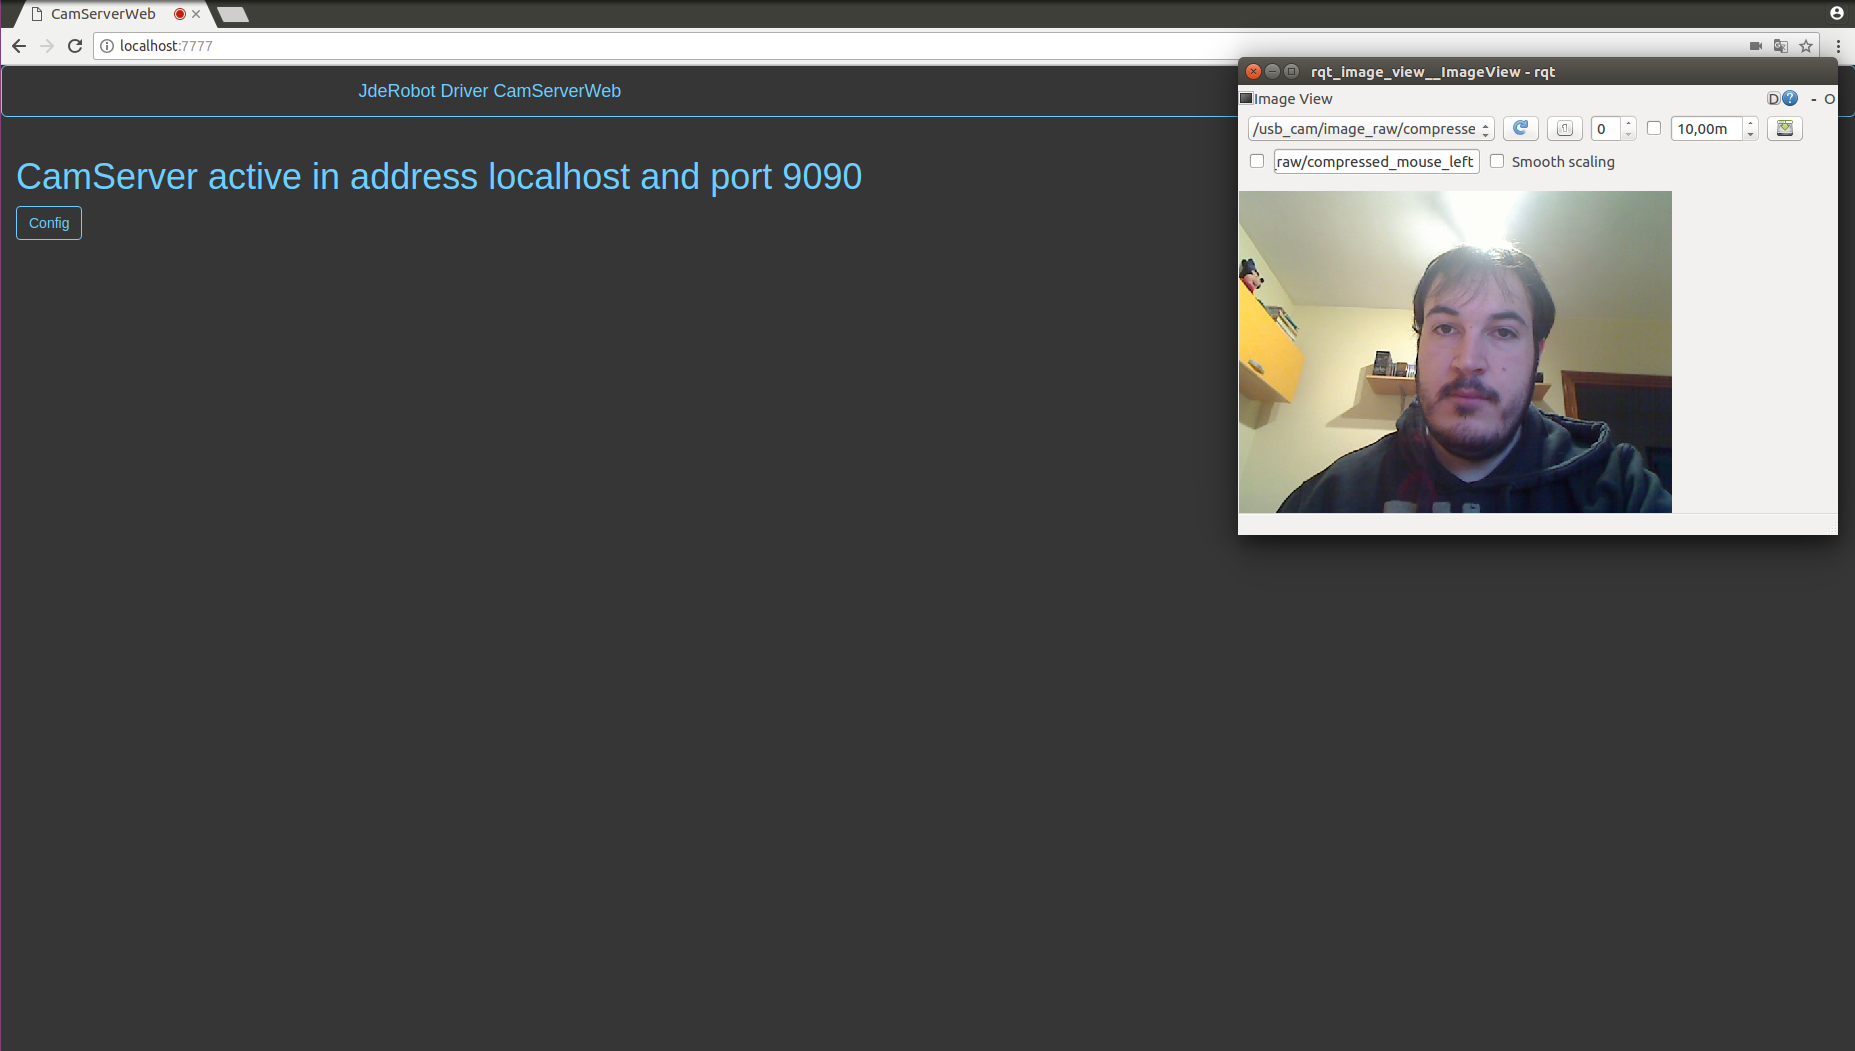
\includegraphics[width=0.8\textwidth]{figures/camservernodejs.png}
    		\caption{CamServerWeb ejecutado en un navegador web}
		\label{fig.testcamserver1}
		\end{center}
\end{figure}
\begin{figure}[H]
  \begin{center}
    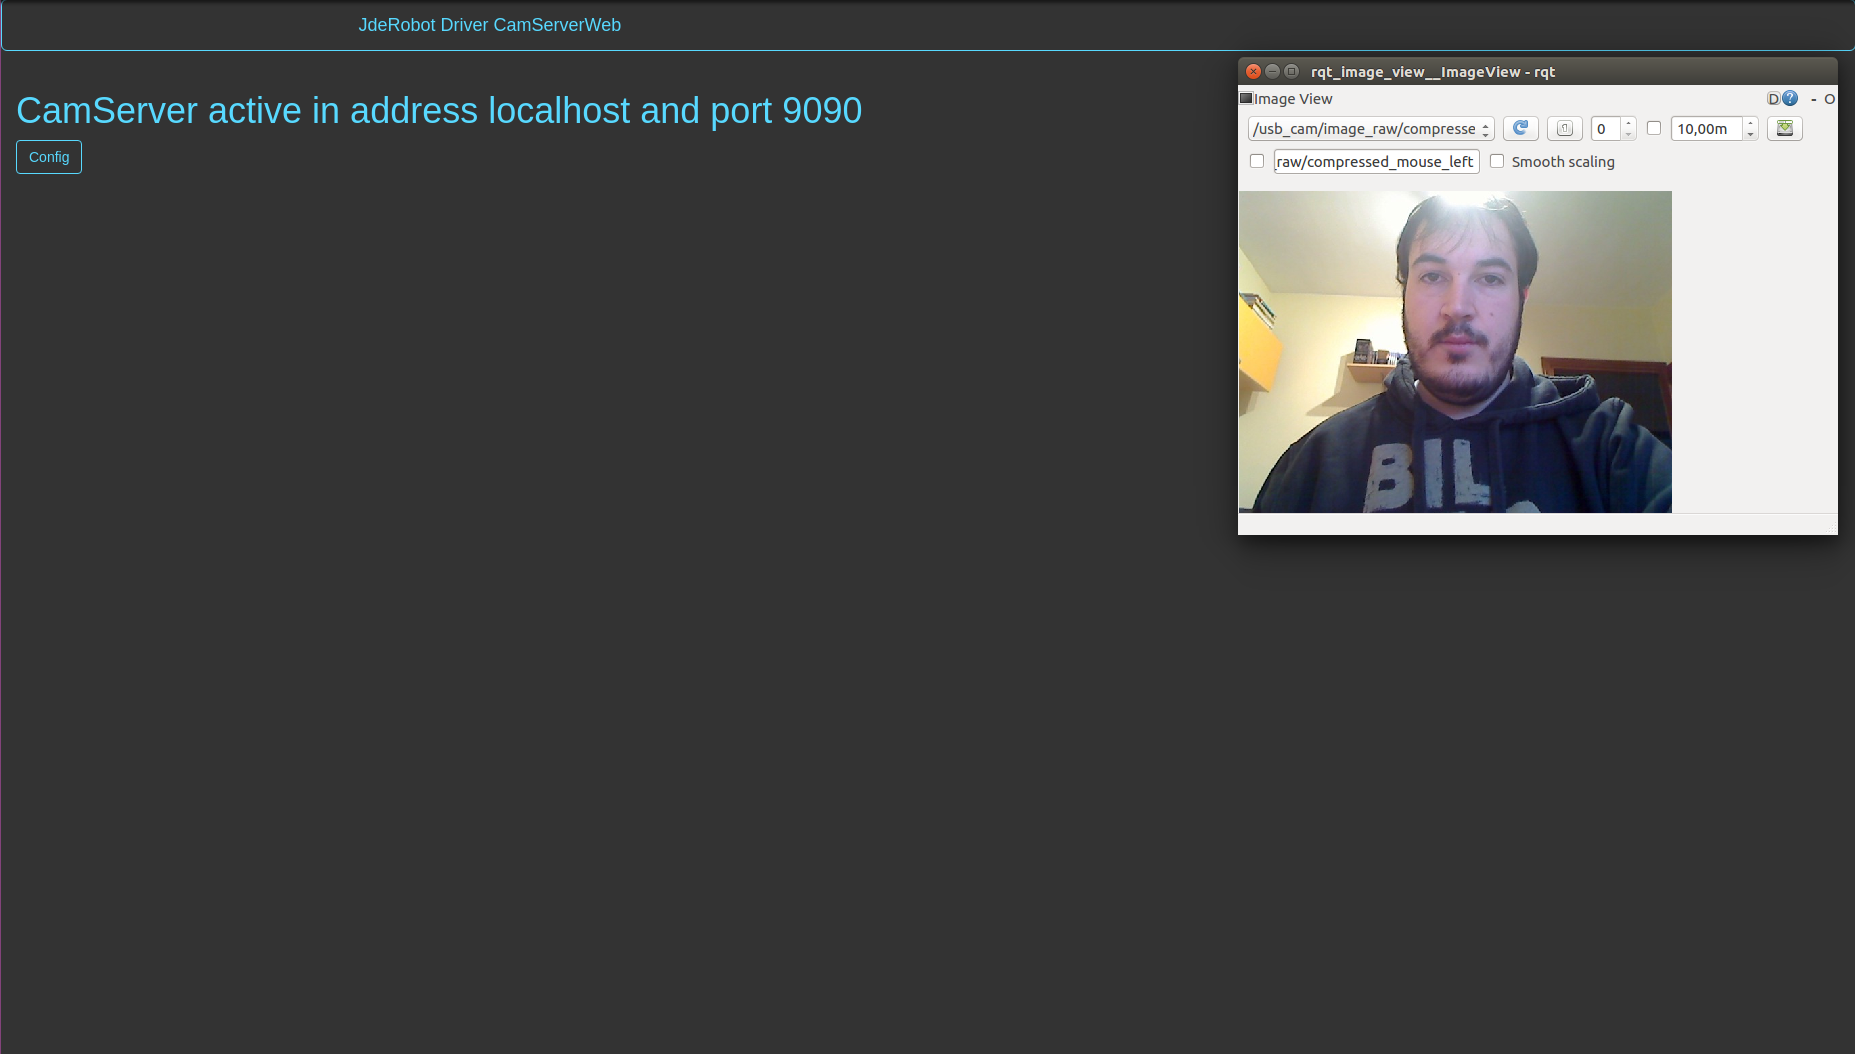
\includegraphics[width=0.8\textwidth]{figures/camserverelectron.png}
    		\caption{CamServerWeb ejecutado en Electron}
		\label{fig.testcamserver2}
		\end{center}
\end{figure}
